\chapter{Implementation}
As evaluated in the last sections this work will proceed to implement TF-DAC-MACS \cite{li2017two} with small adaptions for a practical secure cloud storage system. 

\section{Adaptions and Improvements}
While TF-DAC-MACS satisfy all the requirements it fits not perfectly. To make the scheme more usable, the fix contain that each cipher text need to be secured by a two-factor authentication was removed. In addition, the key generation of the attribute is made more dynamic. Now the attributes do not need to be known in the setup phase but can be created dynamically when an AA admin registers a user. Further, a simple technique to break up TF-DAC-MACS n-of-n threshold policy to DNF-policy in trade-off for performance is proposed. And finally it is argued why the basic access policy of TF-DAC-MACS, even with this proposed extension, renders the usage of numerical attributes and their Boolean comparison inapplicable.

\subsection{Removing The Fix Two-Factor Constrain}
\label{sec:removing-the-fix-two-factor-constrain}
To make \ac{TF-DAC-MACS} more practically applicable the fixed two-factor constrain was removed from encryption, decryption, and the cipher update phase. The two factor identifier $\alpha$ is used by the data owner to restrict the access to the content for certain users. This makes sense since only if the two-factor authentication is in place end-to-end encryption can be garanteed. Users are in charge of generting this two-factor keys, while the attribute keys are created by the AA which has the decryption power of all attributes it created.

This leads to the fact that the underlying \ac{ABE} schemes looses some of it expressiveness. The zero knowledge of the data owner on which individual is able to decrypt the cipher text is broken with the two factor part. Here each user, who wants to decrypt the encrypted content, needs to make an \textit{authentication request} to the data owner to receive the corresponding decryption key. To restore the possibility to let an unknown user group decrypt the cipher text, the two factor part was made optional. To do so encryption, decryption and cipher text update was adapted. The authentication key update will be ignored since it makes no sense to apply it on a non existing authentication key. 

\begin{itemize}
\item \textbf{Encryption:} 
Only the $C_3$ part of the cipher text needs to be updated since it is the only one containing the two factor component $\alpha$.

The original $C_3$:
$$
C_3 = \Big( \prod_{v_{aid_{i}, j}\in W} g^{y_{aid_{i}, j}} \Big)^{s + \alpha} 
$$
is adapted to:
$$
\widehat{C}_3 = \Big( \prod_{v_{aid_{i}, j}\in W} g^{y_{aid_{i}, j}} \Big)^s
$$ 
In addition the $oid$ can be removed from the ciphertext description since it referrers to the data owner ID which is only needed on authentication key update.

\item \textbf{Decryption:}
$SK_W = \prod_{v_{aid_i,j} \in W} SK_{v_{aid_i,j}}$ and $UPK_W = \prod_{v_{aid_i,j} \in W} UPK_{v_{aid_i,j}}$ remain defined in the same was as defined in the paper. 

On decryption the user does not need to generate $UPK_W$ and $SK_{uid, oid}$ anymore. The decryption equation is updated to:

$$
m = \frac{C_1 \cdotp e(H(uid), \widehat{C}_3)}{e(C_2, SK_W)}
$$

Note that the original decryption equation results in the above equation when the two factor part is deducted.

\begin{equation}
\begin{split}
m &= \frac{C_1 \cdotp e(H(uid), C_3)}{e(C_2, SK_W)e(SK_{uid, oid}, UPK_W)} \\
  &= \frac{C_1 \cdotp e\Big(H(uid), \Big( \prod_{v_{aid_{i}, j}\in W} g^{y_{aid_{i}, j}} \Big)^{s + \alpha} \Big)}{e(C_2, SK_W)e(H(uid)^\alpha, \prod_{v_{aid_i,j} \in W} UPK_{v_{aid_i,j}})} \\
  &= \frac{C_1 \cdotp e\Big(H(uid), \Big( \prod_{v_{aid_{i}, j}\in W} g^{y_{aid_{i}, j}} \Big)^{s + \alpha} \Big)}{e(C_2, SK_W)e(H(uid)^\alpha, \prod_{v_{aid_i,j} \in W} g^{y_{aid_i,j}})} \\
  &= \frac{C_1 \cdotp e\Big(H(uid), \Big( \prod_{v_{aid_{i}, j}\in W} g^{y_{aid_{i}, j}} \Big) \Big)^{s + \alpha}}{e(C_2, SK_W)e(H(uid), \prod_{v_{aid_i,j} \in W} g^{y_{aid_i,j}})^\alpha} \\
  &= \frac{C_1 \cdotp e\Big(H(uid), \Big( \prod_{v_{aid_{i}, j}\in W} g^{y_{aid_{i}, j}} \Big) \Big)^{s}}{e(C_2, SK_W)} \\
  &= \frac{C_1 \cdotp e\Big(H(uid), \Big( \prod_{v_{aid_{i}, j}\in W} g^{y_{aid_{i}, j}} \Big)^{s} \Big)}{e(C_2, SK_W)} \\
  &= \frac{C_1 \cdotp e(H(uid), \widehat{C}_3)}{e(C_2, SK_W)}
\end{split}
\label{eq:2faRemoval}
\end{equation}

As shown, no security is threatened since we end up at the same equation as we would do if we had the two factor part included. 

\item \textbf{Attribute revocation:}
The cipher text update key is adapted from

$$
CUK^{ID_W}_{v_{aid_i,j}} = (g^s \cdotp g^\alpha)^{y'_{aid_i,j} - y_{aid_i,j}}
$$

to 

$$
\widehat{CUK}^{ID_W}_{v_{aid_i,j}} = (g^s)^{y'_{aid_i,j} - y_{aid_i,j}}
$$

$\widehat{C}'_3$ now computes as 

\begin{equation}
\begin{split}
\widehat{C}'_3 &= \widehat{C}_3 \cdotp \widehat{CUK}^{ID_W}_{v_{aid_i,j}} \\
&\cdotp \Big( \prod_{v_{aid_{t}, j}\in W, v_{aid_t, j} \neq v_{aid_i,j}} g^{y_{aid_{i}, j}} \Big)^{r} \cdotp (g^{y'_{aid_i,j}})^{r} \\
&= \Big( \prod_{v_{aid_{t}, j}\in W, v_{aid_t, j} \neq v_{aid_i,j}} g^{y_{aid_{i}, j}} \Big)^{s + r} \cdotp (g^{y'_{aid_i,j}})^{s + r}
\end{split}
\end{equation}

It can be shown that $C'_3$ computes to the message $m$ in the same way as shown in equation \ref{eq:2faRemoval}.

\item \textbf{Authentication update:}
Nothing need to change since cipher text do not contain authentication components. 
\end{itemize}

\subsection{Dynamic Secret Key Generation}
Another small adaptation in the \ac{TF-DAC-MACS} scheme was that the attributes for each \ac{AA} does not have to be known on AA initialization. They can as well be created on each users key generation. This reduces the universe of possible attribute values to thous who are actually needed.

\section{Extension To DNF-Policy}
\label{sec:extension-to-dnf-policy}
One big advantage of TF-DAC-MACS is its constant size cipher text. It achieves this by only allowing n-of-n threshold policy. This means that a data owner is only allowed to create \textit{AND} policies to encrypt his content. However, extending this scheme to n-of-m threshold policy is not trivial. To not break any security constrains it was decided to just upload multiple versions of the same cipher text encrypted under different policies. Now, an user only needs to decipher one version of the cipher text to recover the encrypted content. 

To mathematically enable this, the random message $m \in G_T$, which will be the AES-key in the later process, needs to be the same across the different cipher texts. Creating different cipher texts with the same message does not threading security since an attacker still need to find the blinding factor $s$ first to decipher any message. Since this $s$ is chosen for each cipher text randomly and independent of the message $m$ it can be assumed that encrypting the same message with different policies does not result in any security violations. 

Using this approach, access policies in disjunctive normal form (DNF) are enabled for the trade-off of linear cipher text overhead and linear overhead on cipher text updates (both scaling with the number of disjunctions). Formally spoken each Boolean formula can be represented which satisfy the following grammar:

\begin{center}
\begin{lstlisting}[caption={Phseudo gramma for creating a DNF formula},captionpos=b]
root:               or_expression
or_expression:      (or_expression (OR or_expression)* | and_expression
and_expression:     and_expression (AND and_expression)* | attribute_value
attribute_value:    AID.ATTR_NAME:ATTR_VALUE
\end{lstlisting}
\end{center}

So for example "(aa.tu-berlin.de.role:student or (aa.tu-berlin.de.role:professor and aa.tu-berlin.de.institution:dsi))" can be represented by creating a ciphertext the policies "(aa.tu-berlin.de.role:student)" and "(aa.tu-berlin.de.role:professor\\ and aa.tu-berlin.de.institution:dsi)" respectivly. However, not representable is for example: "(aa.tu-berlin.de.institution:dsi and (aa.tu-berlin.de.role:professor or aa.tu-berlin.de.institution:student))".

It must be noted that every Boolean formula can be translated into DNF representation. However, it comes with the disadvantage that each formula, when converted to DNF, will grow exponentially in length. So a formula with $2n$ variables can result in the worst case in $2^n$ DNF clauses. 

\section{Numerical Attributes}
As described by Bethencourt \textit{et. al.} \cite{bethencourt2007ciphertext} we could display numeric values in binary. Each number $x$ is composed of $\lceil log_2(x) \rceil$ attributes. Each of this attributes relate to either a $1$ or $0$ in one position in the binary number representation of $x$. So for example the number $5$ in binary would be displayed as $0101$ and its attribute would be: $x:0***$, $x:*1**$, $x:**0*$ and $x:***1$. 

If a user now wants to create a policy where he challenges a number $x$ to be greater or equal to $3$ he creates a policy: "$(x:1*** or (x:*1** or (x:**1* and x:***1))$". Analogous the policy for $x$ smaller than $4$: "$(x:0*** and (x:*0** or (x:*1** and x:**0* and x:***0))$".

Disadvantage of this representation is that it is limited in space. To display a 32-bit number we must issue 64 attribute values and maintain 64 attribute value keys. It also have to be kept in mind that this formula need to be converted to DNF representation, resulting in a very large overhead of storage and computation.

\section{System design}
A closer look at the system design and how it is implemented will be taken. The system life cycle can be described with the phases: Setup, encryption, decryption, attribute revocation and two-factor-key revocation. Two describe this flow the interaction of each of the five entities present in the system will be sketched. Thouse entities are:

\begin{itemize}
  \item \textbf{Central Server} does the initial setup of the global public parameter used in the later process. It publishes this information on a public bulletin board. Further, the CA is the central entry point to trigger and permit AA creations. It audits the \textit{Authority Identifier} (\ac{AID}) provided by the AA and which should be unique in this system. 

Further, the CA functions as a \textit{Certificate Authority}. It issues a certificate for the GID and RSA public keys of the user. This certificate can be revoked so that the user is not able to obtain new secret keys from the AA or other data owners.
The CA is also the central service that provides all necessary information to the client. Such as public attribute keys, encrypted user private attribute keys and certificates.
 The Central Server is honest-but-curious.
  \item \textbf{Attribute Authority (\ac{AA})} creates the secret keys for its attributes. Attributes are prefixed with the \ac{AID} to ensure uniqueness among the attribute universe. They have decryption power in their domain. Further, they are in charge of revoking attributes. 
  \item \textbf{Cloud Storage Provider (\ac{CSP})} The cloud storage provider provides storage to save the encrypted files. If an cipher text update is needed the CSP updates the cipher text accordingly. 
  \item \textbf{Users} download and decipher ciphertext. They receive attribute secret keys from the AA, GID and certificates from the server and two factor keys from the data owners. The CSP is honest-but-curious as well.
  \item \textbf{Data owner} are specifications of users who can issue two-factor keys to other users. The so called \textit{Two-Factor Key} (\ac{2FA}-Key), adds an additional security layer to the cipher text. It restricts the access to the encrypted plain text to a even smaller select user group.  
\end{itemize}

\todo{Adaptations in system design: CA is certificate authority as well, CSP only saves encrypted keys but not cipher texts. User can not talk directly with each other.}

\subsection{Setup}
The setup summarizes the steps described in \cite{li2017two} such as: Setup, user registration, data owner registration, authority setup, key generation and authentication requests. 

% GPP init
\subsubsection{Generate Global Public Paramter}
The very first step is to create the global public parameters on the central server. Thous parameter are exposed on a public bulletin board and available for each entity in the system. Since they are required in every step it is assumed that the entity downloaded this information in advance. 

% AA setup
\subsubsection{Setup Attribute Authority}
\begin{figure}[!h]
\centering
    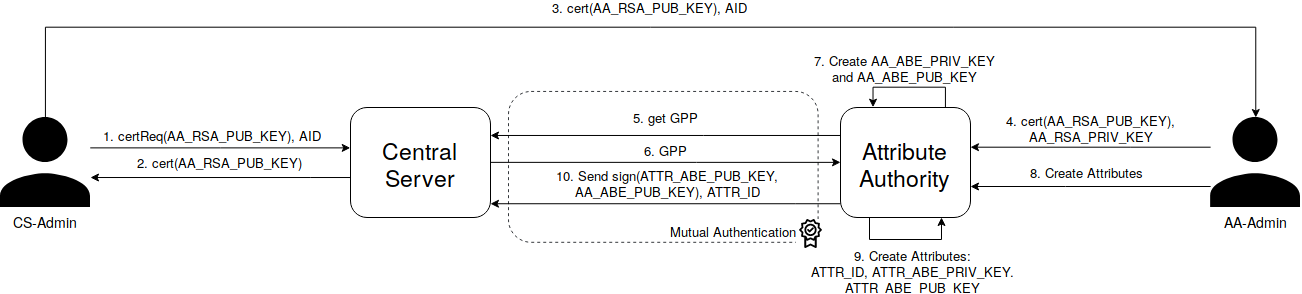
\includegraphics[width=\linewidth]{img/aa_setup.png}
    \caption{Attribute Authority Setup}
    \label{fig:aa-setup}
\end{figure}
An AA is registered, as shown in figure \ref{fig:aa-setup}, with the help of a central server administrator (CS-Admin) and a attribute authority administrator (AA-Admin). As a prerequisite the AA-Admin already created a RSA key pair and send the public component to the CS-Admin together with the desired authority identifier (AID). The AID should be globally unique among this ecosystem so that authority domains can be clearly differentiated. Now the CS-Admin creates a new certificate request embedding the RSA public key of the new AA (1.). The central server checks that the given AID is unique and signs the certificate request (2.). The resulting certificate is passed back to the AA (3.) where it, together with the RSA private key, can be used for mutual certificate authentication. 

The AA-Admin uploads the received certificate and the private key to the AA service (4.) so that it can communicate confident and authenticated with the central server. For each ABE related key generation the GPP are needed, which can now be retrieved over a secured channel, from the CS (5. and 6.). To create attribute keys first an ABE authority key needs to be created (7.) . Now the AA-Admin specifies the attributes by providing the attribute name and values to the service (8.). Internally, the attribute value keys are generated (9.). For each attribute value a ABE key-pair is generated. And to ensure uniques of the attribute identifier it is composed using the following syntax: "<AID>.attr.<Attribute\_name>:<Attribute\_value>". For example the major computer science would be displayed as \\"aa.tu-berlin.de.attr.major:computer\_sience". In the final step, a signed version of the public attribute value keys and authority public key and the attribute identifier are uploaded to the central service (10.).

\subsubsection{Register a user}
\begin{figure}[!h]
\centering
    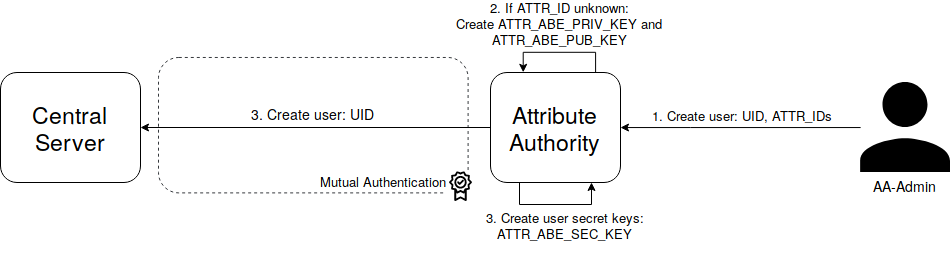
\includegraphics[width=\linewidth]{img/user_register.png}
    \caption{Register a user}
    \label{fig:user-register}
\end{figure}

Figure \ref{fig:user-register} shows the user registration flow. Users are registered by the AA-Admin. He chooses a user identifier (UID) and attributes for the new user (1.).  The AA now checks if all attribute values are already known or if a new attribute value key pair needs to be created (2.). If new attribute values would have been created their public component would also be signed and published to the central server. The user specific attribute secret keys needs to be created (3.). They have the hash of the UID embedded so that on colluding with other users this hash would mesh and no successful decryption would be possible. Finally, the central server is notified for this new user. It just saves the user object for future reference.

\subsubsection{Register a device}
\label{sec:register-a-device}
\begin{figure}[!h]
\centering
    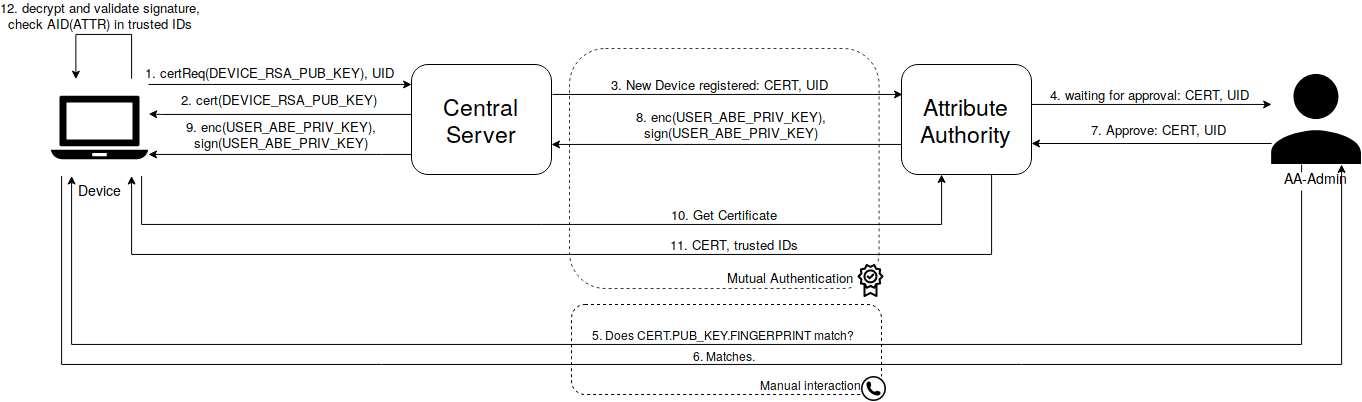
\includegraphics[width=\linewidth]{img/device_register.png}
    \caption{Register a device for a user}
    \label{fig:device-register}
\end{figure}

A device is the first end-system that is able to encrypt and decrypt files in the system. Figure \ref{fig:device-register} shows the rather complex flow for registering a new device. First of all a new RSA key pair on this device is created. These are used for later communication and securing the transmission of the secret attribute keys to the client. 

The device creates a new certificate request embedding its public key as the subject. This certificate request is posted as a pending request under a user object (1.). The central server processes the certificate request, validates that the user with the desired UID exist and returns a certificate for this request to the device (2.). In addition the central service notifies the AA of the user that a new device was initialized by passing the new certificate (3.). The AA-Admin gets notified for this new device and its certificate (4.). He then manually contacts the addressed user and asks him if he registered a new device (5.). They compare fingerprints of the public key of the certificate and the public key of the user’s device (6.). If they match the AA-Admin approves the device (7.). The AA encrypts the attribute secret keys of the user with the public key embedded in the certificate, signs the content and pushes this information to the central server (8.). 

The double check between AA-Admin and user is imported because the central service (since it might try to provide wrong information) might have generated a new RSA key pair, self-signed the certificate request for them and secretly added it as a fake device to a user. If the AA would just send the attribute secret keys along without double checking with the user, the central server would retrieve the attribute secret keys for this user. 

Now the device gets notified that it has been approved and receives the encrypted and signed attribute secret keys (9.). To validate the identity of this secret keys, the device needs to retrieve the certificate of his administrating authority (10.). The device is expected to have the AA address set somewhere in its settings. \footnote{The device can not ask the central server for the certificate or AA address since it retrieves untrustable information.} So the device requests the AA certificate and the trusted AA IDs (11.). The device will only trust attribute secret and public keys coming from a trusted AA ID. If it gets attributes of one of thous trusted AAs, it will request again the certificate of the AA to validate the authenticity of the public and secret attribute keys. 

This is due to the fact that the central server just might overwrite the public attribute keys so that the device encrypts using the tampered keys. Now the central server would only have to use his generated attribute secret keys to decipher the encrypted content. 

In the final step, the device decrypts the attribute secret keys using its private key and validating the signature using the certificate it retrieved (12.). Some might have noticed that the device would just retrieve its attribute secret keys directly from the AA. However, form the view of designing a practical system it makes sense to only have one entry point to retrieve attributes from instead of crawling all trusted AAs periodically. 

\todo{rewrite trusted IDs to trusted fingerprints}

\subsubsection{Register User and Device As An Extern Attribute Authority}
\begin{figure}[!h]
\centering
    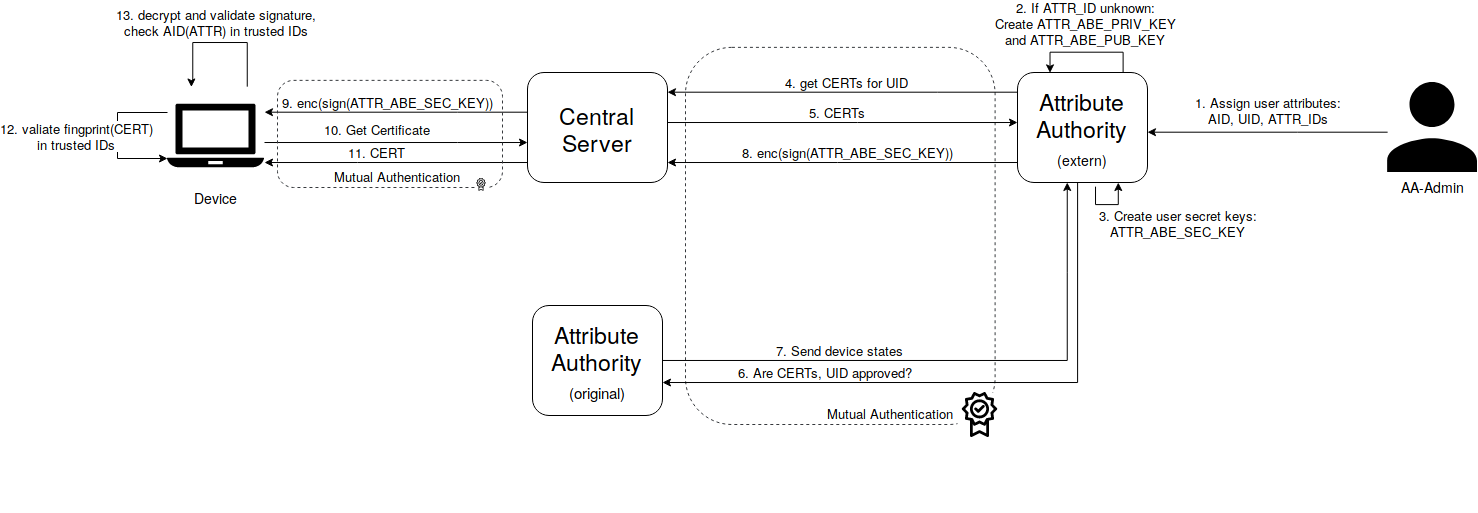
\includegraphics[width=\linewidth]{img/device_register2.png}
    \caption{Register a device for a user as an extern AA. Since this one did not approve the device first handed, it needs to request the original AA for advice.}
    \label{fig:device-register2}
\end{figure}
To enable the feature that other AAs can issue attributes to users managed in other domains, the flow of device registration needs to be adapted.  In its core this process is a merge of thous of figure \ref{fig:user-register} and \ref{fig:device-register}. An administrator will still register the user in this AA addressing the foreign AA. It must be noted that this AA and the addressed AA must be in a trust relation ship. Otherwise the device will reject all attribute keys issued by this AA. This is a security measure to prevent attribute tampering of the central server. With the list of trusted authority IDs the device can retrieve the certificate 

\todo{finish me}

\subsection{Encryption}

\begin{figure}[!t]
\centering
    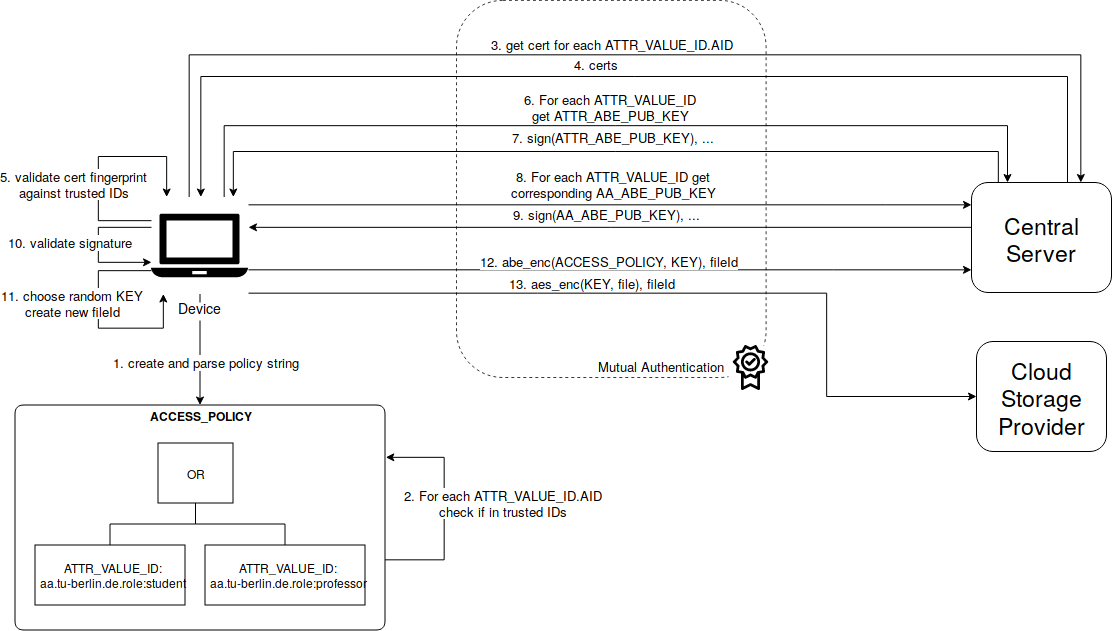
\includegraphics[width=1\linewidth]{img/encryption.png}
    \caption{Encryption phase}
    \label{fig:tfdacmacs-encrypt}
\end{figure}

The encryption process in displayed in figure \ref{fig:tfdacmacs-encrypt}. In the very first step, a user given policy is parsed to create a so called \textit{parsing tree} (1.). Having this parsing tree grantees that no syntax error are present in the parsed policy. For the semantic validation additional steps (2. - 10.) need to made. For each attribute value identifier (ATTR\_VALUE\_ID) we first extract the attribute authority ID. This is done by simply exploiting the syntactical structure of an attribute value. 

Recapualting that an attribute value identifier has the following syntax: \\ATTR\_VALUE\_ID = <AID>.<ATTR\_NAME>:<ATTR\_VALUE>. Knowing this, the attribute ID (AID) can be extracted from the given attribute value. The next steps are done for each attribute value respectively. 

In step 2. it is validated that the given attribute values and their authorities are a subset of the trusted authorities IDs retrieved in the register device process. This is necessary since, the CA can be malicious and might provide tampered attribute public keys which will later be used for encryption resulting in a broken encryption. To counter measure this attack, the device only accepts attribute public keys signed by an trusted authority. The certificate of this authority can be retrieved safely (3., 4.) since the device can validate the fingerprint of this certificate using the given trusted authority fingerprints provided by his originated authority (5.).  

Step 6-9 retrieve the public attribute and authority keys needed for encryption under the given policy. For each request a signed ABE public keys are returned. In step 10. thous signatures are validated given the certificates of step 4. and the trusted authority subset validation of step 5. 

Since all preconditions are fulfilled and all public keys are trusted, the device can proceed to encrypt the content under the given access policy (11.).  To do that, the device first chooses a random key  $K \in G_T$ that is encrypted using the adapted encryption technique of section \ref{sec:removing-the-fix-two-factor-constrain} to create a \textit{file key}. The random element key $K$ is converted into a unique byte array stream and used for symmetric \ac{AES} encryption of the plain text content. To relate file key and cipher text a new random file ID is chosen and attached to both payloads. In step 12. the cipher text is uploaded to the central server to that it can be queried by other clients. A cipher text, as described by TF-DAC-MACS \cite{li2017two}, is composed of an encrypted part (in the paper it is called $C1$, $C2$ and $C3$), the data owner Id, which is only present if two-factor authentication is used (see section \ref{sec:encryption-utilizing-two-factor-keys}), an conjunctive access policy (set of attribute value IDs) and the file ID which references the actuall encrypted content. This last one is uploaded and stored permanentally on the cloud storage provider (13.).  

As mentioned in section \ref{sec:extension-to-dnf-policy} an extension to DNF policy is introduced. To support also OR clauses, the client creates different versions of the file key, each encrypted under a different access policy. As can be seen in figure ref{fig:tfdacmacs-encrypt} the example access policy is composed of two attribute values combined with a disjunction. The client would produce one file key under the policy "(aa.tu-berlin.de.role:student)" and an other for the policy "(aa.tu-berlin.de.role:professor)". Each file keys need to be created using the same key element $K$ so that when decrypted respectively both of them result in the same key that can be used to decipher the encrypted file. As already mentioned, this comes with a performance trade-off in storage and computing power. Cipher text update and cipher text length scales now with a linear overhead for each disjunction, rather then constant as in the original scheme. 

\subsubsection{Encryption Utilizing Two-Factor Keys}
\label{sec:encryption-utilizing-two-factor-keys}
\begin{figure}[!t]
\centering
    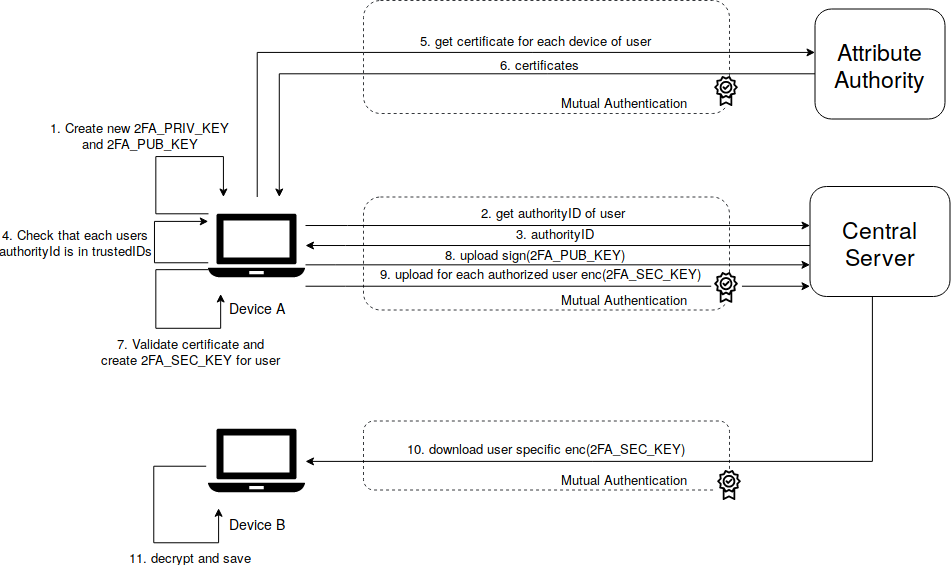
\includegraphics[width=1\linewidth]{img/encryption_2FA.png}
    \caption{Encryption preperation using two-factor authentication}
    \label{fig:tfdacmacs-encrypt-2fa}
\end{figure}

In order to also secure the cipher text utilizing two-factor keys, additional preparation need to be done.  As displayed in figure \ref{fig:tfdacmacs-encrypt-2fa}, first a new two-factor private and public key is created (1.). The private key is kept secret on the device. It will be used later to issue more two-factor authentication keys to other users or revoke two-factor authentication keys. The public key on the other hand will be signed and uploaded to the central server. It serves as input for attribut revokation by an AA. 

For each user that shall receive a two-factor key, the device needs to create a user specific secret two-factor authentication key. To prevent collusion it is made unique for each user using the hash of the user id as a uniqueness source. Before uploading this keys to the central server, the device needs to encrypt them for each user respectively. 

This process is quite complex, since the central server can not be trusted to provide the right user device certificates. It can fake them to retrieve and decrypt the two-factor keys. To cirumvent this, the two-factor issuer askes the central server for the authority ID of the target user (2. and 3.). It is validated, that the retrieved authority ID is an element in the trusted authority ID set (4.). If this check returns success the respective authority is asked directly for the certificate of the devices of the target user (5. and 6.). The certificates are valiadted and finally the user secret two-factor key is created (7.). It is  encrypted using the embedded public keys of the retrieved certificates and uploaded to the central server (9.). Additionally, the two-factor public key is signed and uploaded as well to the central server. The targeted users, will download the encrypted two-factor secret keys (10.) and decrypt them using they secret key (11.).  

The encryption process is then triggered by the two-factor issuer. He can use his privat two-factor key to additionally secure the prepared cipher text. Only users who had the correct two-factor secret key issued and fullfill the access policy can decrypt the cipher text. 


\subsection{Decryption}

\begin{figure}[!t]
\centering
    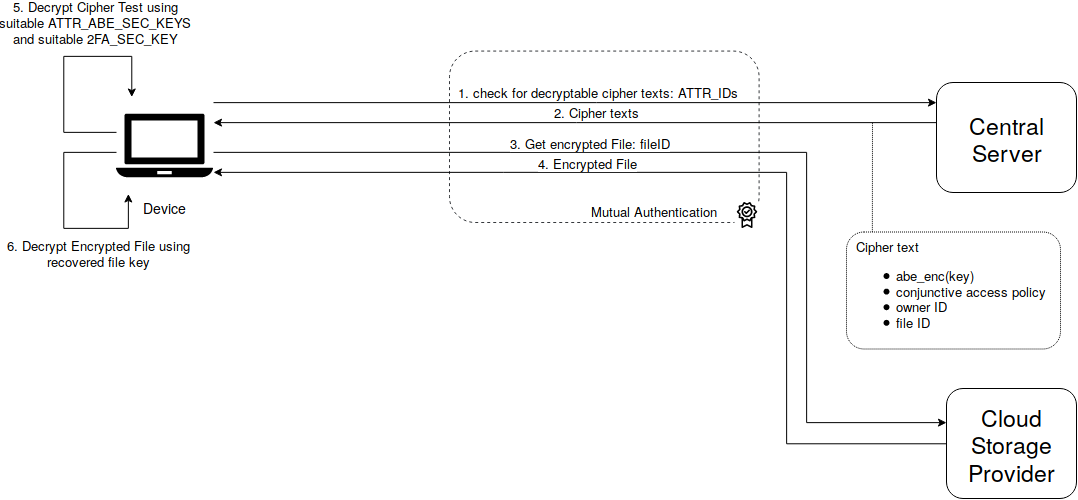
\includegraphics[width=1.0\linewidth]{img/decryption.png}
    \caption{Decryption phase}
    \label{fig:tfdacmacs-decryption}
\end{figure}
Compared to encryption, decryption is rather straight forward. As figure \ref{fig:tfdacmacs-decryption} shows, periodically the device checks if new satisfyable cipher texts are present at the central server. This is done by sending all attribute value IDs for that the devices owns a private ABE key in a query to the central server (1.). It on the other hand checks if any cipher text can be satisfied by a subset of this given attribute set. This can be done by selecting all cipher texts and checking their respective access policies if all elements of this policy are a true subset of the given attribute value IDs from the device. All cipher text that satisfy this constrains are returned (2.).

The device proceeds to extract the file ID from the given cipher text and request this encrypted file from the CSP (3. and 4.). \todo{make integrity checks? Maybe make the file Id to the hash of the file content}. Locally, the cipher text is now decrypted using the user specific ABE private keys issued on device register (see section \ref{sec:register-a-device}) (5.). After the file key is recovered it can be used for symmetric  AES decryption of the encrypted file (6.). 

\subsubsection{Decryption Utalizing Two-Factor Keys}
If a cipher text is additionally secured by a two-factor authentication the user needs to use the suitable two-factor secret key to decrypt the cipher text. Using a wrong or even no two-factor secret key at all will result in a wrong decryption result.

\subsection{Revoke attribute}
\begin{figure}[!t]
\centering
    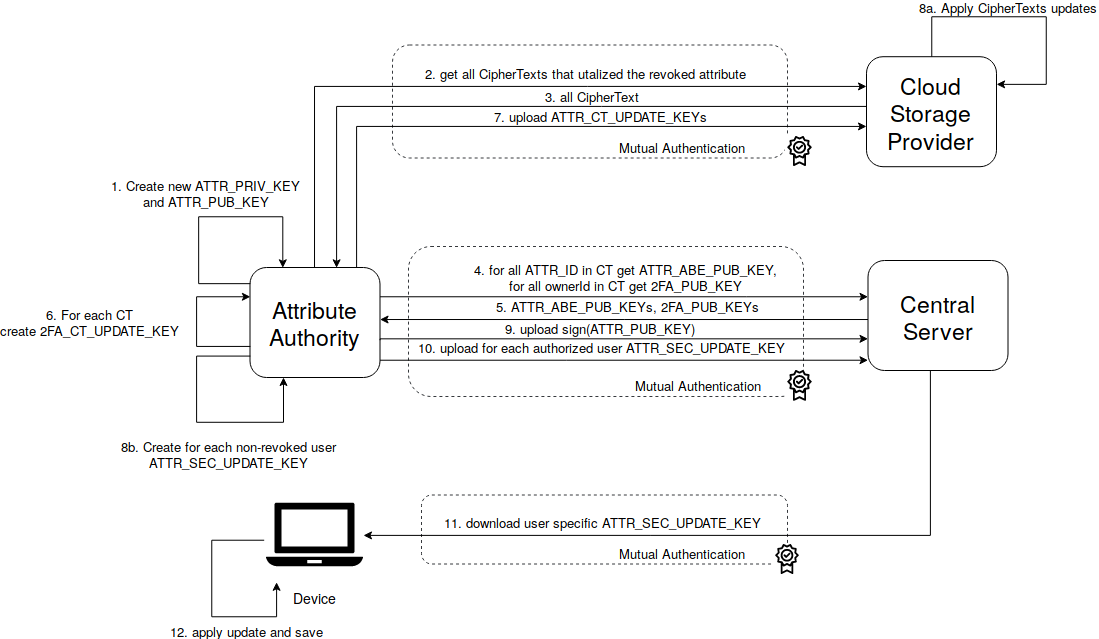
\includegraphics[width=1.0\linewidth]{img/attribute_revokation.png}
    \caption{Revoking an attribute key}
    \label{fig:tfdacmacs-attribute-revokation}
\end{figure}

As displayed in figure \ref{fig:tfdacmacs-attribute-revokation}, a revokation of an attribute key is always initiated by the AA that administeres this attribute. It first creates a new private and public attribute components (1.). In the later steps from this new attribute private key a delta to the old attribute private key is calculated. This delta builds up the core component of the update key that is later distributed to the users and ciphertexts in respective versions. 

In that design the cipher text update key is calculated. To do so, all cipher texts are queried that have the revoked attribute embedded in their attribute policy (3.). To construct a valid cipher text update key, the public attribute keys and the public two-factor keys for each cipher text are needed. They are requested in step 4. and retrieved in step 5. The signature of each of the public keys do not nessecaryly have to be checked since the thread model of the central server only states that the central server will tamper values if it results an significat decryption adventage. However, tampering public attribute keys in that step will result in invalid update keys, which will just render the system inusable. 

Given the public attribute keys, the public two-factor keys and the previous computed delta to the old key the AA can create the two-factor update key (2FA\_CT\_UPDATE\_KEY) for each cipher text (6.). Thouse cipher text update keys are uploaded to the CSP (7.) which starts updating the corresponding cipher texts (8a). 
While the CSP updates the cipher text, the AA proceeds by creating a attribute update key for each users secret key (ATTR\_SEC\_UPDATE\_KEY, 8b). There keys are again user specific. The actual revokation process here is simply to not create an update key for the revoked user. Thouse update keys are uploaded to the central server where they can be discovered by the respective user (10.). Again, this update keys do not have to be signed since they do not contains tamper worthy material nor need they to be encrypted since they contain as a secret the delta to the old version. But if the original secret is known, the new secret can not be calulated. Additionally, the new attribute public key is uploaded in a signed version to the central server (9.). It needs to be tamper proof due it is used on encryption. The central server could act as an own AA to replace the public key with its own, breaking the encryption process due to global decryption power. 

In the last steps, the new update key for the addressed user is downloaded (11.) and applied to the exisiting attribute secret key of the user (12.).

To delete a user all attributes need to be revoked from him. So the above process will be triggered for each attribute the deleted owers owned.

\subsection{Revoke two-factor key}
\begin{figure}[!t]
\centering
    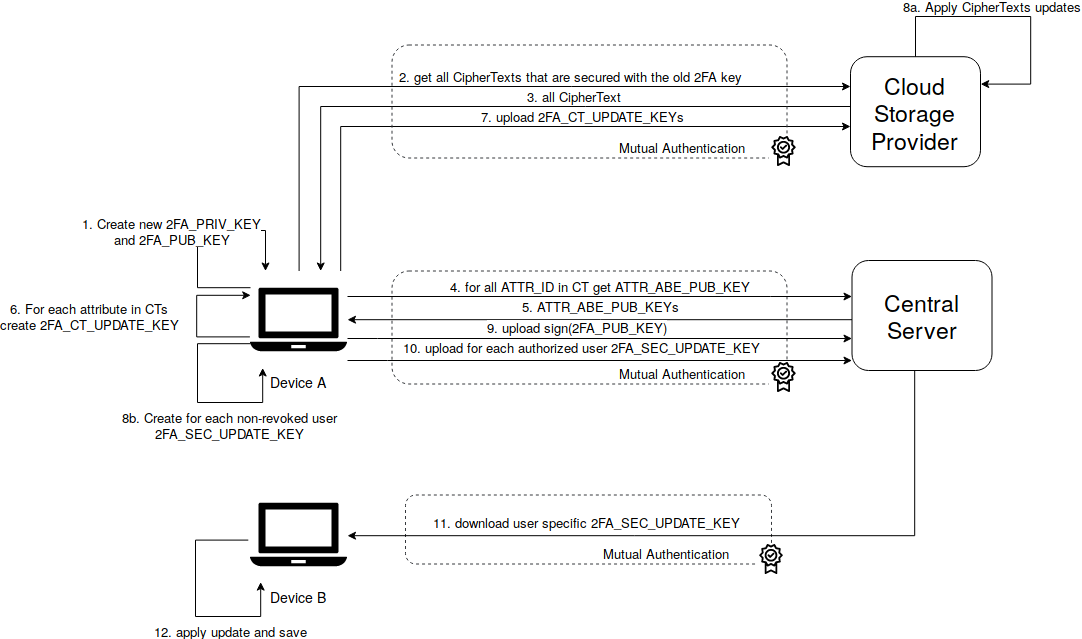
\includegraphics[width=1.0\linewidth]{img/2FA_revoke.png}
    \caption{Revoking two-factor keys}
    \label{fig:tfdacmacs-2FA-revokation}
\end{figure}

The revokation process of revoking a two-factor (Figure \ref{fig:tfdacmacs-2FA-revokation}) authentication from a user follows the same guide lines as the revokation of an attribute. The only difference is that the revokation process is triggered by the user that issued the two-factor key in the first place. 

The data owner frist creates a new two-factor public and private key (1.). Again the delta to the old version is calculated, which makes the update key non-securable obstacle for the later process. Now all cipher text need to be collected from the CSP that where issued by this user and secured by a two-factor authentication (3. and 4.). For each cipher text the attribute policy is extracted and unioned into a set of attribute IDs, which will be send to the central server (4.) to receive the corresponing attribute public keys in return (5.).

Given the new two-factor private key and the attribute public keys, for each cipher text a cipher text update key can be calculated (6.). In Step 7. each of the update keys are send to the CSP where they will be applied to update the old two-factor authentication in the cipher texts (8a). While the CSP applies the update, the client continues with creating for each non-revoked user a user specific update key (8b). The new two-factor public key is uploaded in a signed version to the central server, where it can be used by the AA to create new attribute revokation keys (9.). For each non-revoked user the user update key is uploaded to the central server so that it can be discovered by the respective user, downloaded (11.) and applied to the local user secret (12.).   

\section{Technologies}
To develop the first prototype of the system defined previously we will use the following technology stack:

\begin{itemize}
  \item \textbf{Spring boot}
  \item \textbf{Docker}
  \item \textbf{jPBC} \cite{ISCC:DecIov11}
  \item \textbf{...}
\end{itemize}
\todo{write me}

\section{Problems}

\subsection{En- and decrypting arbitrary data}
TF-DAC-MACS takes as an input for encryption a message $M \in G_T$. Since there is not easy way to reconstruct a message from an element in $G_T$, we have to combine some encryption techniques to encrypt arbitrary data. 

The algorithm first chooses a random $M \in G_T$ and outputs $M$ together with the constructed cipher text. $M$ is then hashed into a byte buffer using \ac{SHA}-256. In the next step we will encrypt our arbitrary data using \ac{AES} and as the key the previous computed hash. 

On decryption first $M$ is reconstructed using the ABE decryption technique and then hashing $M$ again to reconstruct our AES secret key.


\subsection{Distributed infrastructure and parallism}

There are two updates in TF-DAC-MACS: The attribute revokation update and the two-factor key update. If an administrator removes a user from the system all attributes of this user need to be renewed. To make user that also the cipher texts are decryptable by this new attributes it must be updated as well. For that the AA issues an update key which is used by the CSP to calculate the new updated version of the cipher text. 

On the other hand there is the two-factor revokation. Here a user wants to revoke the two factor key access from a specific user. To do so he issues update keys to each non-revoked user and an cipher text udate key to the CSP to also update the resepctive cipher texts.

While this both operations are by design assoiative, they depend on transactional execution of each operation. But this constrain can not be provided in a distributed intfrastructure. 

For an two-factor revokation all relevant attribute public keys are needed. If at the same time this public values are updated by an AA a malfunctioning two-factor update key will be calculated. For example assume the following execution order:

\begin{enumerate}
\item The Data Owner downloads the attribute public key in version 1 and computes the update key 2FA-Update
\item AA issues Attribute Public Keys in Version 2 and uploads this one to the CA and computes Update Key ATTR-update
\item AA sends ATTR-update Key to the CSP which also triggeres the update process for all cipher texts which are encrypted using this given attribute 
\item In parallel Data Owner sends 2FA-update Key to the Cloud Storage Provider (CSP) which starts the update process of all 2FA Ciphertexts that are secured using the old two-factor key
\item Ciritical is now this step where the CSP updates a cipher text using 2FA-update which is already updated using ATTR-update rendering the ciphertext unusable
\end{enumerate}

\begin{equation}
C''_3 = 
\left(\prod_{v_{aid_{t},j} \in W, v_{aid_{t},j} \neq v_{aid_{i},j}} g^{y'_{aid_i,j}} \right)^{(s+\beta+r')}
\cdot 
\underbrace{
    \left(g^{y'_{aid_i,j}}\right)^{(s + \alpha + r')} 
    \cdot 
    \left(g^{y_{aid_i,j}}\right)^{(\beta - \alpha)} 
}_\text{due to of different basis exponents can not be aggregated} 
\label{eq:wrong-update}
\end{equation}
In equation \ref{eq:wrong-update}, $g^{y'_{aid_i,j}}$ refernces the revoked attribute and $\left(g^{y_{aid_i,j}}\right)^{(\beta - \alpha)}$ the two factor update key $UAU_{aid_i,j}$ for this revoked attribute. In that case the data owner used the old attribute public key $g^{y_{aid_i,j}}$ to compute $UAU_{aid_i,j}$.

The very first step to countermeasure this kind of problems is to detect this issue. This is done by assigning each key a version. If a private ABE key gets created it gets the initial version $0$ assigned. Each other key that is derivatived from this private key ends up with the same version. 
In the same way the user attribute secret keys and two-factor secret keys are created. Both of them need to be updated if a revocation takes place. 

On the other hand, cipher texts contain for each attribute used in its policy the version of the used attribute public key as well as the version of the public two-factor authentication key that was used to additionally secure it. Only keys that are present in the same version as the used public encryption keys can be used to decrypt this cipher text. Each other key will be rejected.

Update keys contain a target version and increment the version of the applied key. If applied in a cipher text it will increment the version of the targeted two-factor component or targeted attribute component. 

Having this versioning in place, the CSP can now detect any wrong issued update to a cipher text. It will check that the given update is applicable to the given cipher text and only if this check returns true, it will proceed to update the cipher text. Next steps will be to notify the update issuer about the conflicting versioning and request a updated update key. 

Since updates on keys need to be incremental and strictly sequential, the CSP or user need to wait until a suitable update was issued to him.  